\chapter{Machine Learning}
Machine learning is playing a fundamental role in natural language processing
and computational linguistics. The impact is so significant that one of key note
speakers of ACL 2012, Mark Johnson, predicted that in 50 years from now NLP/CL
will not exist as a research field and will be emerged as two different
fields:(1) machine learning and (2) logic. This chapter is dedicated  to subset
of models in machine learning that can play a role of bridge between logic and
machine learning. This chapter provides the building material for a new
direction of research so called \textit{Representation Learning} which enables
us to transfer information from logical forms such as predicate-argument form to
vector space (beside many other advantages which we will discuss).
Most of current models in machine learning are designed to work in vector space
therefore it is an important achievement to be able to work with type of
information which is in other forms or representations by first transferring
them to vector space. Working with logical forms in vector space helps us to use
many available knowledge bases and lexicons with available machine learning
models which is crucial for relation discovery. I will skip discussing classical
machine learning problems to emphasis more on new relevant topics. 
I will first briefly review artificial neural networks and then motivate and
define the task of representation learning. In next chapters, we will
need the materials provided in this chapter to understand the undergoing
research about relation discovery.
\section{Artificial Neural Networks}
\label{sec:ml-ann}
Before diving into different methods of representation learning, it would be
useful to briefly review the architecture, applications and learning algorithms
of artificial neural networks (ANN). ANNs can be used for variety of
applications in machine learning: classification, clustering, dimensionality
reduction,\ldots ~. What makes ANN important for us is their ability to do many
of mentioned tasks jointly. Its layer-wised architecture very well fits to the
idea of multi-task learning. Different layers of an ANN can have different
objectives and can share information with other layers through parameter
sharing. First I discuss about elements and architecture of ANNs and then we
will very briefly review \textit{backpropagation} and \textit{stochastic
gradient descent} as we need them to understand the mechanism of learning in
ANNs.

Artificial neural networks have old history in the domain of machine learning.
They are inspired from the mechanism humans learn via their neural networks. The
basic element of this network is a neuron which takes a weighted input signals and by applying an activation function
on this input, the neuron will output a signal. 
 Neurons are usually arranged in
layers and receive input from the neurons from the previous layer and send their
outputs to the next layer. The combination of different layers and using
different activation function with different degree of non-linearity is enabling
ANNs to learn non-linear functions.
A common mathematical model for neuron in ANNs is shown in
\eqref{eq:neuron} and visually in \autoref{fig:neuron-model}.
\begin{equation}
\label{eq:neuron}
\begin{split}
x^{l-1} \mbox{~: input vector of size~}n  \mbox{~and layer~}l-1
\\
w^{l,l-1} \mbox{~: weight vector of size}~n~ \text{from layer}~l-1 \text{~to
layer}~l
\\
y_{j}^{l} \mbox{~: output value of neuron~}j  \mbox{~at layer}~l\\
y_{j}^{l} = f(\sum_{i=0}^{n} w_{i,j}x_{i}^{l-1})\\
\end{split}
\end{equation} 
Activation functions can be
usually either of functions in the list below:
\begin{description}
\item[linear function] ~~ $f(x)=ax+b \mbox{~where}~ a,b \in \mathbb{R}$
\item[step function] ~~ $ f(x)=1 \mbox{~if~} x > \theta \mbox{~else~} f(x)=0
\mbox{~where~}\theta \in \mathbb{~R} \mbox{~is a constant threshold} $
\item[tangent hyperbolic] ~~ $f(x)=tanh(x)$
\item[Log-sigmoid] ~~ $f(x)=\frac{1}{1+e^{-x}}$
\end{description}

    \begin{figure}[h!]
  \caption{A model of neuron}
  \centering
    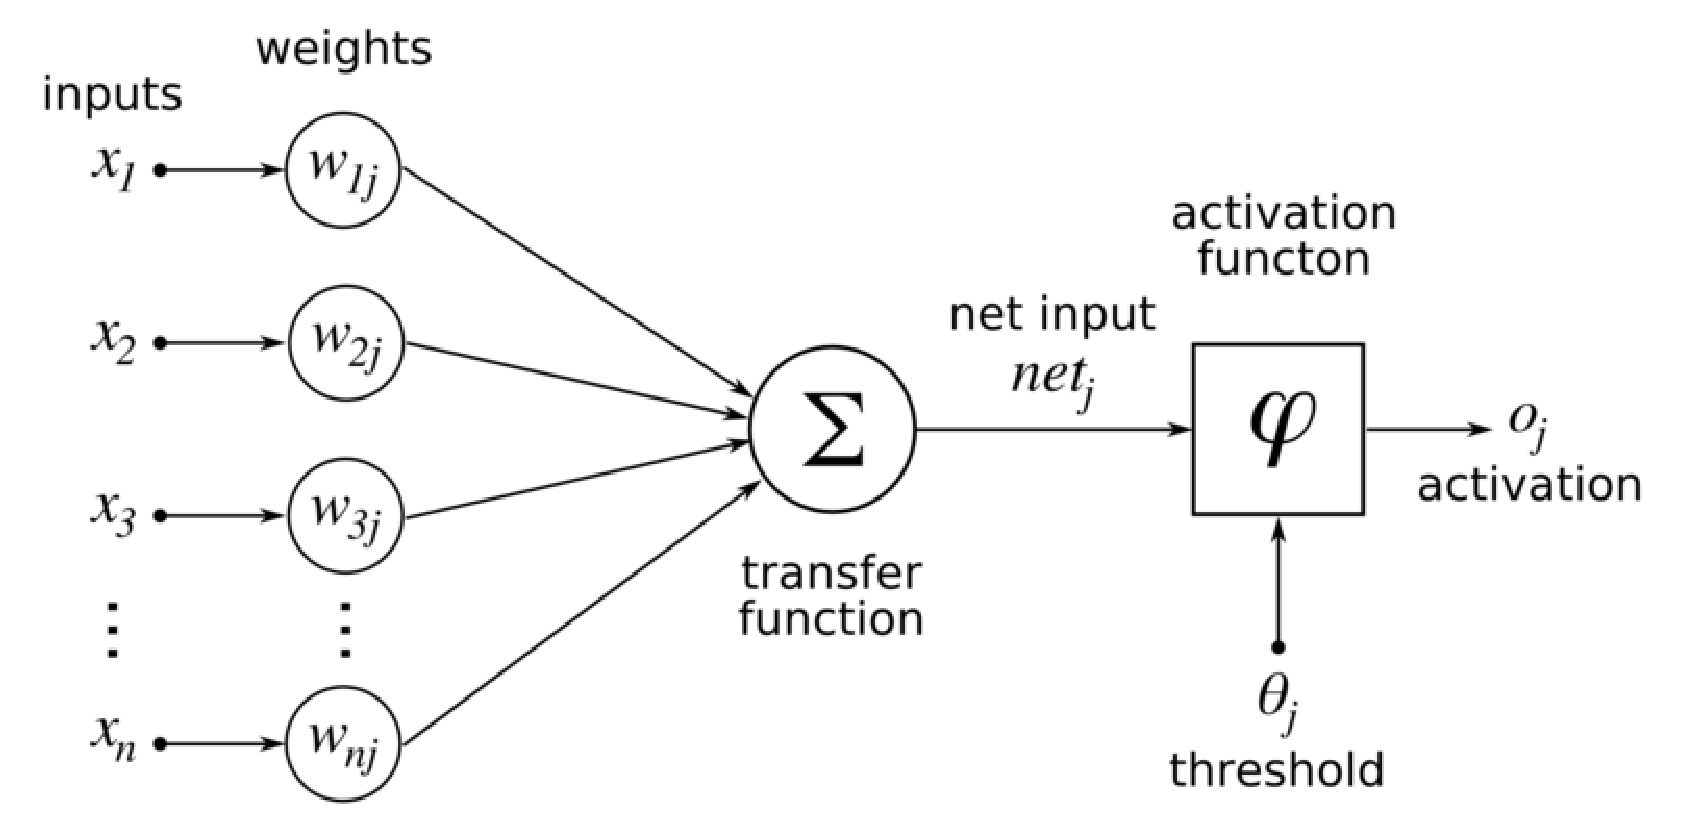
\includegraphics[width=0.8\textwidth]{neuron-model.eps}
    \label{fig:neuron-model}
\end{figure} 

The type of ANNs matters mostly for us in this research are
networks which neurons are arranged in ordered layers and there is no feedback
from a deeper layer  to the layers in the back. The first layer is usually for
unsupervised pre-training of objects, then a layer for adding non-linearity
comes and finally we have an axillary classification or ranking task.
 \begin{figure}[h!]
  \caption{A Neural Language Model proposed by Bengio et al.}
  \centering
    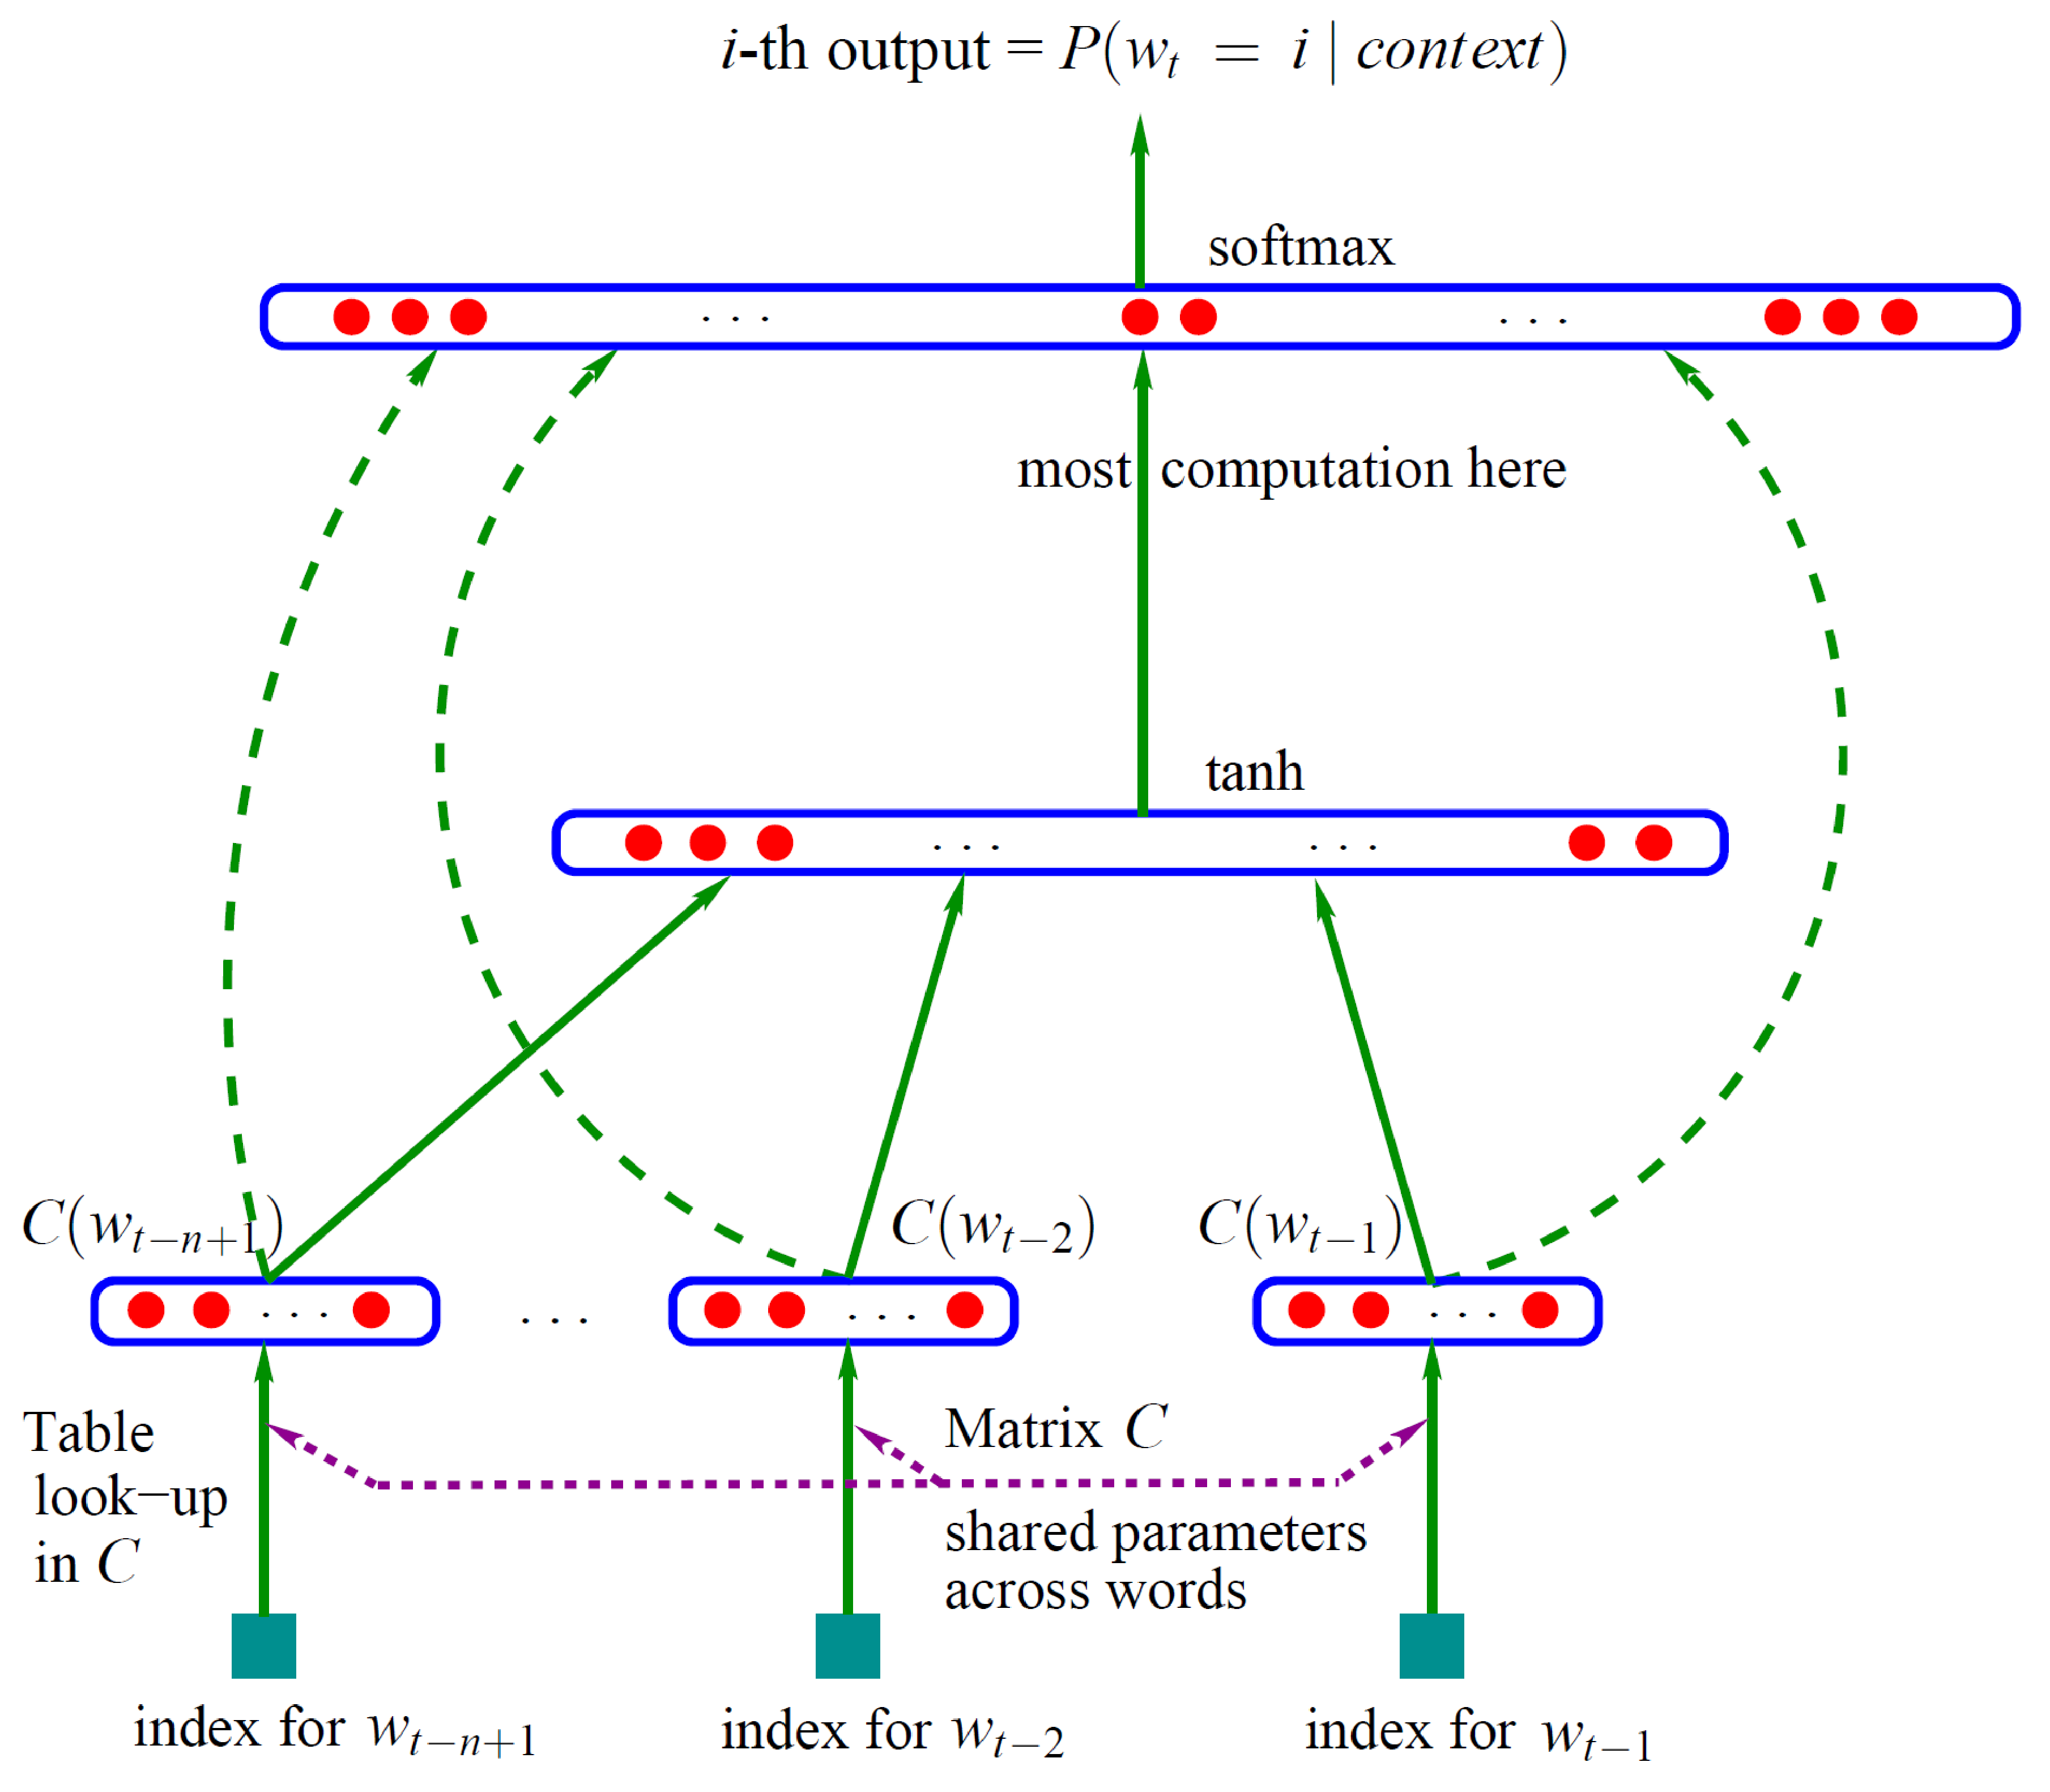
\includegraphics[width=1\textwidth]{ann.eps}
    \label{fig:ann}
\end{figure} 
 In \autoref{fig:ann}
 we can see a neural architecture proposed by Bengio et al. \cite{Bengio2003}
 which works as language model. This model takes n-grams as input and predict
 the probability of the next word. The first layer is hot-one representation of
 sequence words, $w_{t-n+1}, \ldots ,w_{t-2}, w_{t-1}$ and then the layer for
 unsupervised pre-training of words comes.
 Learned features of words will be combined together with \textit{tanh} layer
 and finally we will have a \textit{softmax} layer which outputs probability of
 all words as the next word, $w_t$, in the sequence. Later we will see more details about 
 different layers of this ANN but
 the main question that arises here is how to learn parameters of such a network
 in order to make good predictions and induce meaningful features for words.

There are two main approaches for learning parameters of a single supervised
layer. By supervised layer we mean that true outputs/predictions are available
for training the parameter of the layer. :
\begin{description}
  \item[Online learning] \hfil \\
    To optimize the parameters, we
    iterate over all points in the training dataset and calculate the layer
    predictions for input. In each iteration, we update the weights in order to
    decrease the difference between the predicted output and the true output for
    each point. This forms an objective function (error function) which can be
    minimized by gradient descent, by calculating error derivatives and update
    weights to decrease them.
    Since each data point can change the parameters, we call this algorithm an online learning algorithm.
  \item[Batch learning] \hfil \\
  In this approach, unlike the previous approach, first we calculate the
  predicted outputs of whole dataset and form the error function and try to
  minimize the error derivative for whole dataset. Since we update the
  parameters after observing all points in the training dataset we call this
  approach batch learning.
  
  \item[Stochastic Gradient Descent] \hfil \\
  The idea of SGD is to make best out of both previous ideas. Neither updating
  after each datapoint nor after all points, SGD makes small batches in each
  iteration, each usually contains only 100 datapoints, and calculate error
  derivatives and update parameters for each batch.
  
  
\end{description} 

Since we now know how to train a single supervised layer, other layers of a
network can be trained using \textit{backpropagation}. Parameters of the network
will be randomly initialized and then by choosing one of the approaches above we
can start by learning the last layer, since we have the output for that. After
updating the last layer, it works as the output of the layer before it and we
can use the same strategy to train its parameters. Likewise, we continue
training of other layers. The criteria for stopping the algorithm can be either
maximum number of iterations or when parameters don't change from after some
iterations.

After introducing ANNs we will focus more on the idea of unsupervised
pre-training in the next section. I show the generalization of this idea using
other methods and motivates it as a very crucial step in many NLP tasks.

\section{Representation Learning}
\label {sec:repr-learning}

In this chapter, we will define and justify the task of
\emph{Representation Learning} and we will see different families of methods for
inducing word representation and its application in NLP.

In machine learning specially in industry, most of the labor is dedicated to
\emph{Feature Engineering}. Extracting informative features is the crucial part
of most supervised methods and it is done mostly manually. While many different
applications share common learning models and classifiers, the difference in
performance of competing methods mostly goes to the data representation and
hand-crafted features that they use. This observation reveals an important
weakness in current models, namely their inability to extract and organize
discriminative features from data. Representation learning is an umbrella term
for a family of unsupervised methods to learn features from data. Most of recent
works on the application of this idea in NLP focus on inducing word
representations. \emph{Word representation} is a mathematical object, usually a
vector, which each dimension in this vector represents a grammatical or
semantical feature to identify this word and is induced automatically from data
\cite{Turian2010b}. Recently, it has been shown in \cite{Turian2010b} and \cite{Collobert2011} that using
 induced features can be helpful to improve state-of-the-art methods in 
different NLP tasks. It seems that relation extraction can also benefit from such features since similar tasks like 
semantic role labeling has been shown to benefit from
induced word representations. In ~\autoref{ch:text-kb} and
~\autoref{ch:ent-link} I will show two applications of it, (1) direct usage for relation discovery and
(2) word feature generation which can be used in current relation discovery
systems as well as other NLP applications.
In the next two sections, two major families of representation learning methods
will be shortly reviewed.

\subsection{Distributional Representation}
\label{sec:distl-repr}
In distributional semantics, the meaning of a word is expressed by the context
that it appears in it \cite{Harris1981}. Features that are used to represent the
meaning of a word are other words in its neighborhood as it is so called the
context. In some approaches like LDA and latent semantic analysis (LSA), 
the context is defined in the scope of a document rather than a window around a
word. To represent word meanings in via distributional approach, one should
start from count matrix (or zero-one co-occurrence matrix) which each row
represents a word and each column is a context. The representation can be
limited to raw usage of the very same matrix or some transforms like
\emph{tf-idf} will be applied first. A further analysis over this matrix to
extract more meaningful features is applying dimensionality reduction methods or
clustering models to induce latent distributional representations. A similar
clustering method to k-means is used in \cite{Lin2009} to represent phrase and
word meanings and brown clustering algorithm \cite{Brown1992} has been shown to
have impact on near to state-of-the-art NLP tasks \cite{Turian2010b}. 


\subsection{Distributed Representation}
\label{sec:disted-repr}
Distributed representation has been introduced in the literature for the first
time in \cite{Bengio2003} where Bengio et al. introduced a first language
model based on deep learning methods\cite{Bengio2009b}. Deep learning is
learning through several layers of neural networks which each layer is
responsible to learn a different concept and each concept is built over other
more abstract concepts. In the deep learning society, any word representation
that is induced with a neural network is called \emph{Word Embedding}. 
In contrast to raw count matrix in distributional representations, word embeddings are low-dimensional, dense and real-valued vectors.
 The term, \textbf{`Distributed'}, in this context refers to the fact that
 exponential number of objects (clusters) can be modeled by word embeddings.
 Here we will see two famous models to induce for such representations. One
 family will use n-grams to learn word representation jointly with a language
 model and the other family learns the embedding from structured resources.
In \cite{Collobert2008a}, Weston and Collobert use a non-probabilistic and
discriminative model to jointly learn word embeddings and a language model that
can separate plausible n-grams from noisy ones. For each word in a n-gram, they
combine the word embeddings and use it as positive example. They put noise in
the n-gram to make negative examples and then train a neural network to learn to
classify positive labels from negative ones. The parameters of neural network
(neural language model) and word embedding values will be learned jointly by an
optimization method called \emph{Stochastic Gradient Descent} \cite{Bottou2010}.

A hierarchical distributed language model (HLBL) proposed by Mnih and
Hinton in \cite{Mnih2009} is another influential work on word embeddings. In
this model a probabilistic linear neural network(LBL) will be trained to 
combine word embeddings in first $n-1$ words of a n-gram to predict the $n_{th}$
word.

Weston-Collobert model and HLBL by Mnih and Hinton are evaluated in
\cite{Turian2010b} in two NLP tasks: chunking and named entity recognition. With
using word embeddings from these models combined with hand-crafted features, the
performance of both tasks are shown to be improved.
 
\subsection{Representation Learning of Knowledge Bases}
\label{sec: repr-learning-kb}
Bordes et al. in \cite{Bordes2011} and \cite{Bordes2012} have attempted to use
a neural distributed model to induce word representations from lexical resources
such as WordNet ~\cite{Fellbaum1998} and knowledge bases (KB) like Freebase
~\cite{Bollacker2008} .
In Freebase for example, each named entity is related to another entity by an instance of a specific type of relation. In
\cite{Bordes2011}, each entity is represented as a vector and each relation is decomposed to two
matrices. Each of these matrices transform left and right-hand-side entities
to a semantic space. Similarity of transformed entities indicates that the
relation holds between the entities.  A prediction task is defined to evaluate
the embeddings. Given a relation and one of the entities, the task is to predict
the missing entity. The high accuracy (99.2\%) of the model on prediciton
of training data shows that learned representation highly captures attributes of
the entities and relations in Freebase.

Two major models are proposed in \cite{Bordes2011} and \cite{Bordes2012} to
learn features in continuous  vector space from a Knowledge Bases(KB) which information is
usually represented in form of triples of $(e_{i},r_{k} , e_{j} )$ where $e_{i}$ and $e_{j}$ are $i_{th}$ and $j_{th}$ entities related
 by a binary relation of type $r_{k}$. The purpose of the models is to induce a vector space and associate
  each entity or relation to an embedding vector or a matrix.
  The dimensions of such an embedding vector are supposed to reflect a set of informative features of entities and relations.
   
   In the first model, \textbf{structured embeddings(SE)}, entities are modeled as \textit{d}-dimensional vectors.
    An associated vector to the $i_{th}$ entity, $e_{i}$, is $E_{i} \in \mathbb{R}^{d}$. Each relation $r_{k}$  
    is decomposed to two operators each represented as $d \times d$ matrix, $ R_k = (R_{k}^{left}, R_{k}^{right})$. 
    These operators transform the left and right entities to a new space induced by each relation and by using 
    a $p$-norm measure  (L1 norm in this work) they associate a similarity value or a score to each triple. 
    This similarity value is being calculated by
    Equation ~\eqref{eq:sim}. 
    \begin{equation}
    \label{eq:sim}Sim(E_{i}, E_{j}, R) = ||R_{k}^{left}E_{i} - R_{k}^{right}E_{j} ||_{1}
    \end{equation}
    The similarity between transformed entities works as a score to measure the strength of a relation holds between two entities. 
      
    Using the idea of contrastive learning , the model will be trained to increase similarity of 
    embeddings for a positive triple (a triple which exists in the KB) or lowering its rank among other training samples
    and decrease the similarity of embeddings when the relation doesn't hold (negative triple) or raising its rank . 
    For each positive triple, two negative triples will be generated by randomly alternating the right entity or left entity with other entities.
    Inspired from large margin methods a constraint is introduced on the model
    that forces negative triples to have lower associated similarity value  than correspondent 
    positive triples by a large margin. In \autoref{fig:bordes2011} a schematic
    view of model is presented.
    
    \begin{figure}[h!]
  \caption{Neural Distributed Model to Learn Structured Embeddings (SE)}
  \centering
    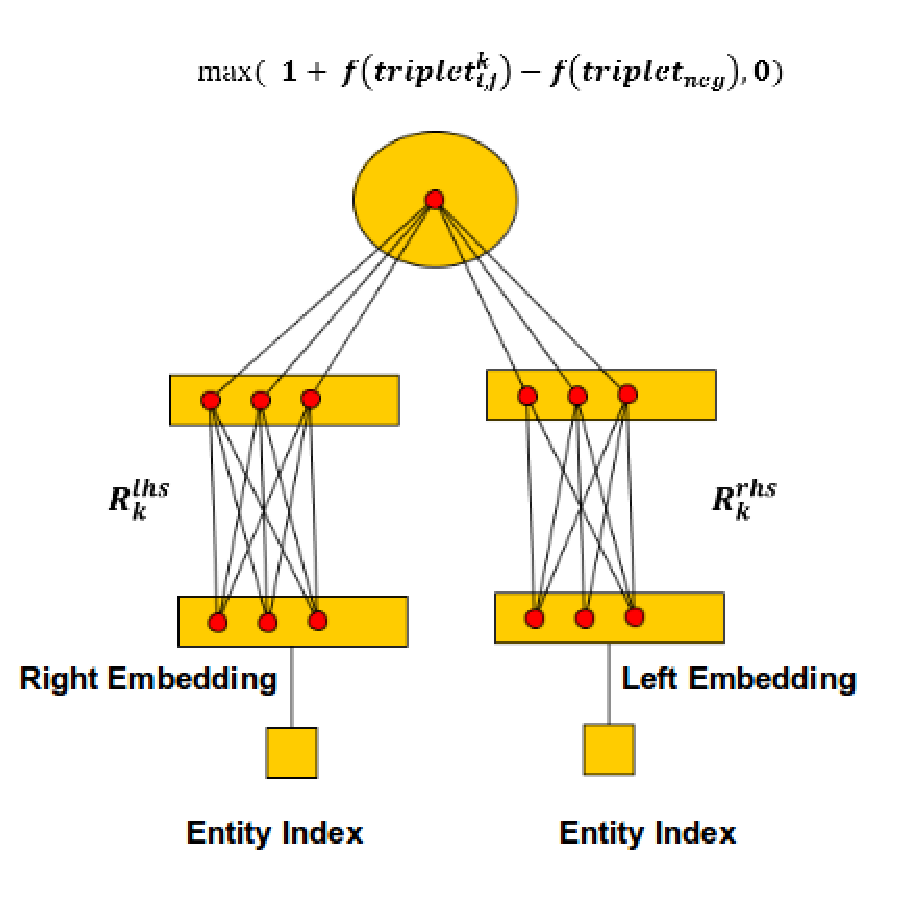
\includegraphics[width=0.5\textwidth]{bordes2011.eps}
    \label{fig:bordes2011}
\end{figure} 
    The second model, \textbf{Semantic Matching Energy using Bilinear layers(SME-Bil)}, 
    is using a different representation for relations,weighted bilinear
    transformation of embeddings and  dot product similarity function instead of L1 norm. 
    In this model, each relation is represented by a \textit{d}-dimensional vector $R_{k}$ same as entities. 
    For triple $(e_{i},r_{k} , e_{j} )$ , the model combines the weighted transformation of each entity embedding with 
    the weighted embedding of relation using element-wise vector product. as it is shown in Equation ~\eqref{eq:bil}.
    \begin{equation}
    \label{eq:bil} E'_{left} = (W_{i} E_{i}) \odot (W_{k} R_{k}) + b_{left}
    \end{equation}
    $W_{i}$ and $W_{k}$ are $d \times d$ weight matrices and $b_{left}$ is a $d$-dimensional bias vector. 
    The same equation holds for transforming the right entity embeddings to $E'_{right}$. Finally, the associated score for the triple
     can be calculated by dot product of $E'_{left}$ and $E'_{right}$ which is
     shown in Equation ~\ref{eq:dot}. \autoref{fig:bordes2012} is used by Bordes
     et al. to sketch SME-Bil model. Similar constraints to the first model are also applied to this model and 
     both models can be trained by stochastic gradient descent (SGD) which we
     introduced in \autoref{sec:ml-ann}.
    
   \begin{equation}
    \label{eq:dot} Sim(E_{i}, E_{j}, R_{k}) = -E'_{left}E'_{right}
   \end{equation}
     \begin{figure}[h!]
  \caption{Neural Distributed Model to Learn Structured Embeddings (SME)}
  \centering
    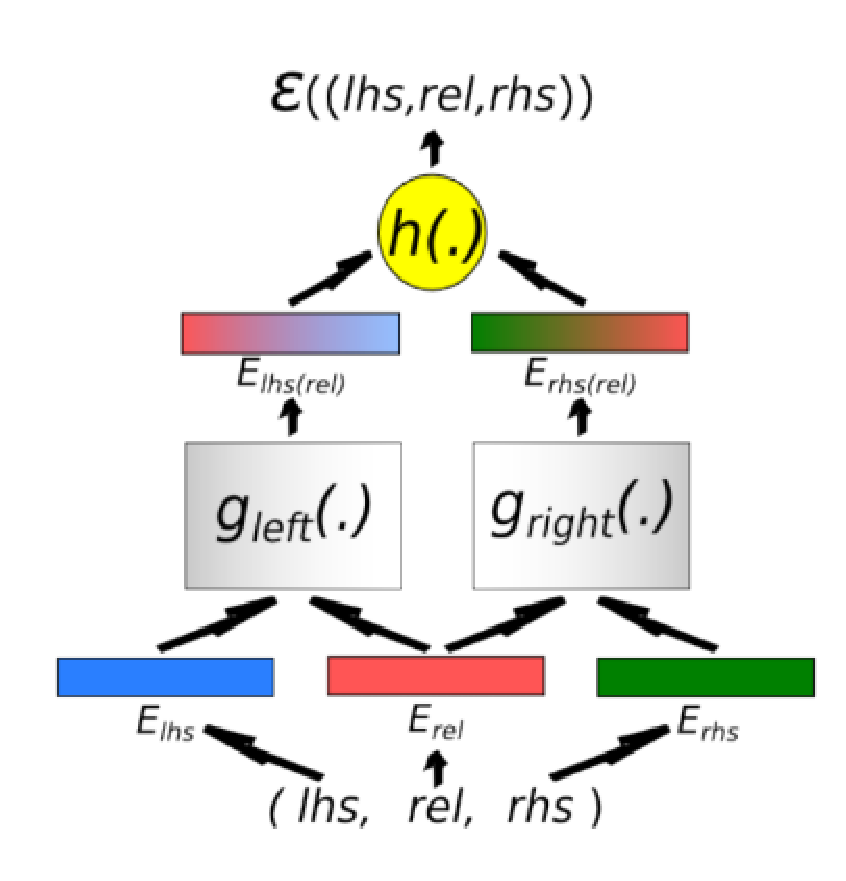
\includegraphics[width=0.5\textwidth]{bordes2012.eps}
    \label{fig:bordes2012}
\end{figure} 
   

\iffalse
\section{Bayesian Non-Parametric Models}
\label {sec:bnp}

\subsection{Introduction}
\label{ssec:intro}
One of the most important contributions of Machine Learning to Natural Language
Processing and Computational Linguistics is to provide variety of statistical frameworks for modeling
 different aspects of language. Modeling makes the data more interpretable and is trying to represent 
 it in a compact way. From language modeling to syntax and semantics, 
 computational models are needed to first describe and then predict the certain phenomena in language. 
 Here we address a family of models which are trying to be less dependent on human choice or 
 trial and error schema for choosing best parameters and are called Bayesian nonparametric models (BNP).
 
\subsection{Model Selection with BNP Models}
\label{ssec:model-sel}
A traditional approach for model selection is to have a set of models and then try to fit 
these models on the linguistic data by tuning and inferring the parameters of them [2]. 
It is more like a search in possible space of models and their parameters to find the best setting. 
Therefore, it is necessary to have a criterion to select the models to see which one is better 
explaining the data and have the prediction power. There are two main features that any criterion 
should consider necessarily. First is the accuracy of prediction (model fitness) and it ensures that 
the model is well-defined and second is the complexity of model [1,2]. 
Let us define these terms in a mathematical language so we can introduce a Bayesian framework for modeling. 
The data is often a set of data points which could be represented as vectors or is in more 
complex structure like a graph or an ordered sequence. For simplicity we first start with 
data point or vector representation of data. Let us define the data as:
\begin{equation}
\label{eq:data}
D = y_1,y_2,\ldots,y_n
\end{equation}


The model could express predictions by the likelihood which is in this form:
\begin{equation}
P(D|\theta,m)
\end{equation}

You see that the predictions are conditioned on the model and a specific parameter in this way. 
In a fully Bayesian model, one should specify the range of parameters or more precisely 
a distribution over possible parameters should be determined beforehand [2]. 
This could be done by adjusting the prior and then we can incorporate the role of all possible parameters 
to predictions weighted by their importance. Here one can notice that the set of parameters are fixed.
\begin{equation}
P(D|m) = \int \! P(D,\theta|m) \, \mathrm{d}\theta = \int \!
P(D|\theta,m)P(\theta|m) \, \mathrm{d}\theta.
\end{equation} 

One can see in this formula that the prediction is average over all parameters weighted by prior. 
Each model is a generative process of data which gives us a joint distribution of hidden and observable variables. 
Each data point is drawn from a distribution of observable variables conditioned on 
hidden variables (parameters of model) and hidden variables are drawn from a prior distribution [1]. 
To infer the posterior distribution (distribution of hidden variables conditioned on observable variables) 
we can reverse the generative process. 
Instead of generating a data point from the distribution we look for the model that more likely explains 
the generation of the data. [1,4]
The second important aspect of model selection is measuring the complexity of the model. 
If we have two models with about same level of fitting, we favor the one that is simpler since it 
performs better generalization for unseen data. Knowingly as Occam’s razor rule having 
less complex model helps avoiding overfitting to the observed data. Bayesian 
framework naturally favors simpler models by putting prior over parameters 
and penalizing unnecessary complexity of the model [2]. 
One can cleverly ask how much complexity is required for a particular data and how can 
we adapt our modeling to change predictions in the case of having new unseen data? 
The answer of Bayesian nonparametric modelling (BPN) to this problem differs to all previous models 
in a way that instead of comparing different models with different complexities it tries to fit 
a single model on the data which changes its complexity by seeing new data. 
While previous methods have fixed set of parameters, BNP assumes an infinite number of parameters. 
It is like that BNP has infinite amount of money (parameters) in the bank and whenever 
the data is more expensive (more complex) it spends more money to model the data. 
Actually \textit{nonparametric} could be misleading  since they have infinite number of parameters 
but only activate a finite subset of them in the learning phase.  
Another point of view is to see a BNP model as information channel which parameters are bandwidth of this channel. 
As data grows bigger, more information should be captured by the model so it increase its bandwidth 
(uses more parameters) [2].
There are several families of BNP models available due to different tasks and structure of data and 
hidden variables. In following, we enumerate these families shortly and then we
go more in depth for one of them.

These groups of models are [1,4,2]:
\begin{enumerate}
  \item Classification and Regression task (Gaussian processes)
\item Clustering (Dirichlet processes and Chinese restaurant processes)
\item Density estimation (closed link to clustering)
\item Ordered discrete sequences data (infinite HMM)
\item Tree structured data or Hierarchical data (Adaptor grammar, infinite PCFG,
Kingman’s coalescent, HDP)
\item Overlapping clusters and factor analysis (Indian Buffet processes)
\end{enumerate}

\subsection{Clustering (Dirichlet processes and Chinese restaurant processes)}
\label{ssec:bnp-chinese}

\fi

    